% Chapter Template

\chapter{Implementation} % Main chapter title

\label{Chapter5} % Change X to a consecutive number; for referencing this chapter elsewhere, use \ref{ChapterX}

\lhead{Chapter 5. \emph{Implementation}} % Change X to a consecutive number; this is for the header on each page - perhaps a shortened title

%----------------------------------------------------------------------------------------

\section{Introduction}

This chapter will discuss in detail, the implementation of the proposed Android client application, and the server application that accompanies it.

With the system already designed out and with a list of set features, I started exploring various coding patterns I could use to implement my design.

\subsection{Architecture and Design Patterns}

Design patterns are reusable solutions to commonly occurring problems in software design. The use of tried and tested design patterns is important in software because it stops programmers from making the same mistakes, and also speeds up development time as you no longer need to 'reinvent the wheel' with every software engineering project.

Picking the correct design pattern for the problem can prove troublesome, and choosing the wrong ones can lead to inefficient solutions, such as unnecessary duplication of code.

For this project, 'MVC' was used heavily in both the client and server side application.

\subsubsection{Model-View-Controller (MVC)}

Model-View-Controller is a well known software design pattern for implementing user interfaces. The design follows three interconnected parts:

\begin{itemize}
	\item Model - holds the application data, and logic  for accessing and manipulating this data.
	\item View - holds logic that displays the aesthetic view to the user. It can also contain mechanisms of receiving user input and passing that input along to it's controller.
	\item Controller - holds controller logic that accesses data from a model and passes it to a view. It can also update a models state with new information, and update the view as the model is updated.
\end{itemize}

Figure \ref{fig:mvc} shows the MVC architecture.

\begin{figure}[htbp]
	\centering
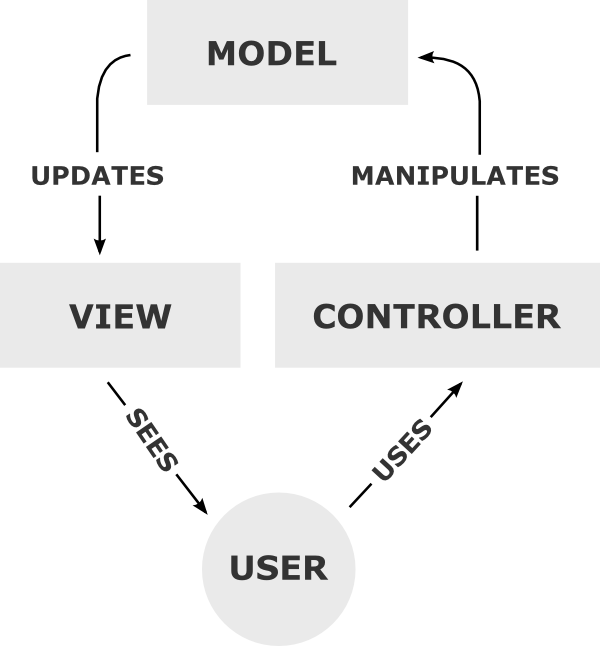
\includegraphics[width=\textwidth,height=\textheight,keepaspectratio]{Figures/MVC.png}	
		\rule{35em}{0.5pt}
	\caption[Model View Controller Diagram - \cite{wikiMVC}]{Model View Controller Diagram - \cite{wikiMVC}}
	\label{fig:mvc}
\end{figure}

The server application makes heavy use of certain aspects of MVC. Models are created for data storage and the transport of the objects from server to client. Controllers are also created to design restful web requests that the client can use to request the data models remotely. Views are not used in the project because no user interface is required for the web server.

The Android client application also uses this pattern, with the controllers requesting data from the remote server, using models to formulate the data into the right structure, and displaying the data in views.

\subsubsection{Component Pattern}

The component pattern is also used in the client application. The business logic is decoupled into separate components. A component is a typical manager class with helper functions that can be accessed anywhere in the applications code.

This allows the Android views to access different components and their functionality easily through a component manager.

\section{Project Setup}

A difficult part of the implementation was the development of both the client and the server at the same time, where features of the client are dependant on features of the server and vice versa.

For example, I could not implement the appointment information features of the client application until the server was able to send that information to it. I was also not able to test certain features of the server until the client had implemented ways of authenticating and sending the requests that the server would respond to.

\subsection{Emulating Requests}

To solve this problem, I used a tool called Postman to emulate the client requests to the server. 

Postman is a simple web application that allows you to design RESTful web requests very easily and send them to a server. By doing this, I was able to design and test the requests I needed easily.

This meant I could focus solely on implementing the basic server features without having to develop the Android application alongside it. I later found that this was also an invaluable method of testing server features when problems occurred.

\begin{figure}[htbp]
	\centering
		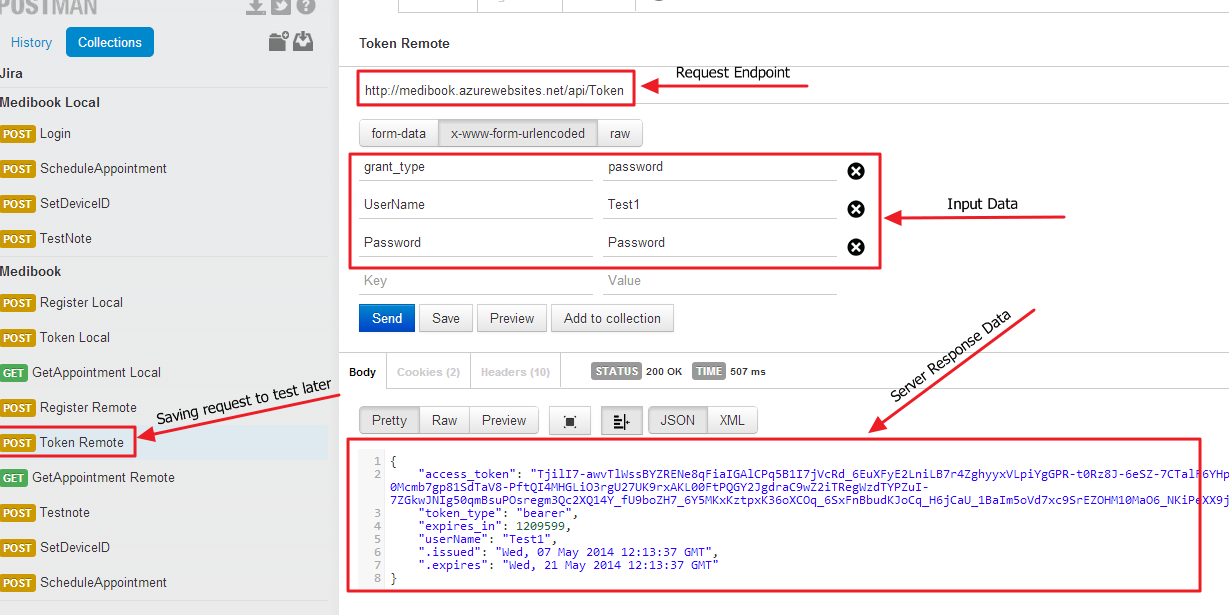
\includegraphics[width=\textwidth,height=\textheight,keepaspectratio]{Figures/Postman.png}
		\rule{35em}{0.5pt}
		\caption[Screenshot showing the use of Postman]{Screenshot showing the use of Postman}
	\label{fig:postman}
\end{figure}

\subsection{Organising Code}

A feature in most modern programming languages (including C\#) is the idea of modular design. This concept emphasises the separation of code functionality into interchangable modules. These modules can then reference other modules easily, and makes sharing code simpler.

Early on in the implementation stages, I found that I was having to duplicate some code and data values in both the client and the server application. This caused many unnecessary issues. For example, I would sometimes change one value and forget to change the other.

To solve this problem, I structured all of my code into separate modules so that they could easily be shared with both my client codebase and my server codebase. 

I organised the code into the following projects:

\begin{itemize}
	\item Medibook.Client.Android - The Android application that focuses entirely on Android specific design. \textit{References the Medibook.Client library.}
	\item Medibook.Client - The client library that contains all business logic that is shared with Android and IOS implementations. \textit{References the Medibook.Shared library.}
	\item Medibook.Server - The server application. \textit{References the Medibook.Shared library.}
	\item Medibook.Shared - The shared library that is shared between the Medibook.Client and Medibook.Server projects.
	\item Medibook.Testing - A unit-testing library that tests specific features of the client application and ensures they are working correctly.
\end{itemize}

With this modular setup, I was able to develop reusable code with no duplication, and allowing for a future iOS app to use the same business logic as the Android app.

With my projects setup, I began developing the basic infrastructure that that both the server application and android application would use.

\section{Server Structure}

Using the Asp.Net framework, the majority of the server's structure was already pre-ordained with a strong emphasis on using the Model-View-Controller design pattern. The server was therefore structured into two components:

\begin{itemize}
	\item Controllers - Containing the business logic and servicing all RESTful API request endpoints.
	\item Models - The data models for storing in the database and designing the structure of sent request data.
\end{itemize}

The server application did not have views because no interface was required for the prototype.

Most of the server implementation was done using controllers, as methods defined in a controller would become a web service endpoint which web-requests from the Android application could execute.

\begin{figure}[htbp]
	\centering
		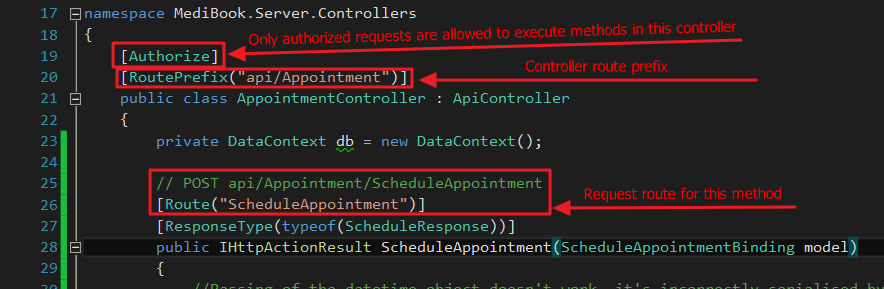
\includegraphics[width=\textwidth,height=\textheight,keepaspectratio]{Figures/ServerController.png}
		\rule{35em}{0.5pt}
		\caption[Example of a controller code showing authorised and routed requests]{Example of a controller code showing authorised and routed requests}
	\label{fig:servercontroller}
\end{figure}

Figure \ref{fig:servercontroller} shows the basic setup of an Asp.Net controller, including routing and authorisation. Every request method in this controller requires an authorised token.

\subsection{Authentication}

Authentication is supported by Asp.Net, so it's implementation was not as tricky as first thought in my original design.

By adding the [Authorize] attribute to a controller or individual request methods, Asp.Net recognises that this request (or all requests within the controller) requires authentication in order to access it.

To authorise requests, authorisation keys called 'Tokens' must be added to the requests authorisation header. If the authorisation header is missing or incorrect, the server will end the request and respond with the HTTP request code '401 Unauthorized'.

All requests sent to the server application require authentication, except the login and register requests, to ensure that patient data is kept secure.

\subsection{Routing}

When the server receives a request from the client, it will be in the form of a url. Asp.Net automatically parses this url into segments, in the form of '{controller}/{action}'.

After the segments have been parsed, it finds the correct controller defined with the controller segment, then the correct action method with the action segment and executes it, returning the output to the sender.

As a working example, if the client sent a request of 'Appointment/Schedule' would tell Asp.Net to look in the Appointment controller for the Schedule request method.

\subsection{Request Methods}

After the request has been routed to the correct method, the data needs to be de-serialised into a binding model.

This binding model defines the structure of the request, specifying the data types for each input parameter. It also provides validation tools to ensure that the data is input correctly.

\begin{figure}[htbp]
	\centering
		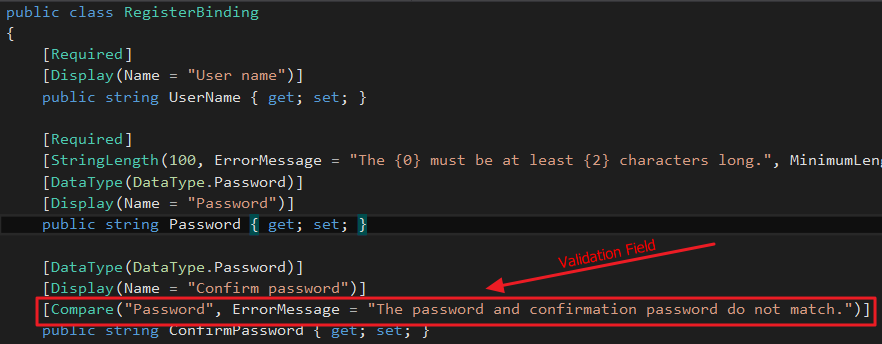
\includegraphics[width=\textwidth,height=\textheight,keepaspectratio]{Figures/bindingmodel.png}
		\rule{35em}{0.5pt}
		\caption[Example of a binding model associated with the register account request]{Example of a binding model associated with the register account request}
	\label{fig:bindingmodel}
\end{figure}

If the binding model is invalid for any reason, the server will end the request and respond with the HTTP status code '400 Bad request'. Error messages will also be returned if available, giving the request sender a reason as to why the request failed.

After the binding model is successfully validated, the request can be carried out the result is returned to the sender.

\subsection{Data Storage and Retrieval}

For data to be stored and retrieved easily, I used the Entity Framework library which integrates easily with ASP.Net and eliminates the need for most of the data access code. 

Two methods are available for database development when using Entity Framework; code first and database first. Code first allows you to let Entity Framework create and setup the database as you write your data models. Database first allows you to use entity framework to generate data models from an already existing database. For quick development, the code first method was chosen for this project.

\subsubsection{Data Models}

Data models work the same way as binding models, in that you design properties with data types for the data to bind to.

You can even use data models as binding models, which allowed me to reuse the same data models to serialise and de-serialise the data when sending to and from the client. I found however, that this was not always a good solution, as some data models have extra information that the client doesn't need (for example, the password property for a user model should not be sent to and from the client, especially when it is a different user).

Entity Framework data models also allow you to assign attributes to the properties such as '[key]' to modify it's behaviour as a primary key when stored in the database.

The best and most useful feature in entity framework is the automatic handling of foreign keys. If in one data model, you wish to reference a different data model, you can set the data type of that property to the data model's type and Entity Framework will do the rest of the hard work. This eliminates the need for any sql queries to fetch other data models that correspond to the foreign keys.

\begin{figure}[htbp]
	\centering
		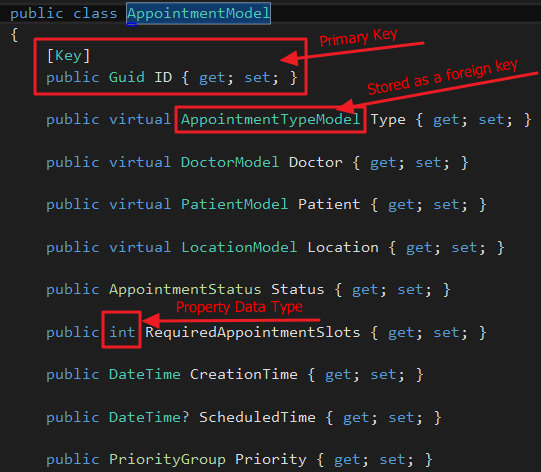
\includegraphics[width=\textwidth,height=\textheight,keepaspectratio]{Figures/EFModel.png}
		\rule{35em}{0.5pt}
		\caption[Example of an Entity Framework Data Model]{Example of an Entity Framework Data Model}
	\label{fig:efmodel}
\end{figure}

All data models were first designed by hand using entity relationship diagrams, however as the project progressed, these models became dramatically different as new features were added.

\begin{figure}[htbp]
	\centering
		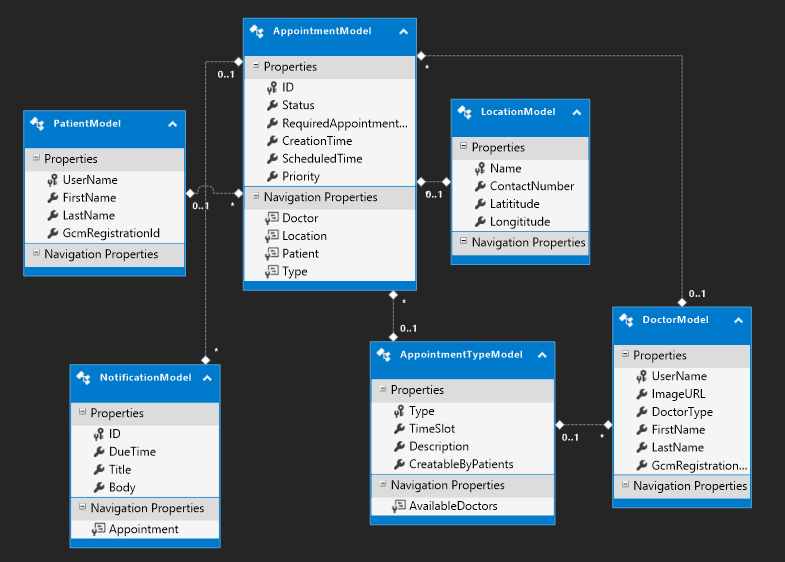
\includegraphics[width=\textwidth,height=\textheight,keepaspectratio]{Figures/database.png}
		\rule{35em}{0.5pt}
		\caption[The Final Entity Relationship Diagram]{The Final Entity Relationship Diagram}
	\label{fig:erdiagram}
\end{figure}

\subsubsection{Data Context}

When using Entity Framework, you must also create a data context.

This data context maps all of the entities and relationships that are defined in each data model to a database using the 'DbSet' class, allowing you to insert, update and delete data easily.

The data context also stores changes to the database transactionally, meaning that changes will only be written when calling the 'SaveChanges' method. This allows for changing the models with ease and not adding any performance issues as it writes unnecessary changes.

Using the data context, you can also query the data easily using LINQ.

\subsubsection{LINQ}

LINQ allows for the easy querying and updating data sets through C\# code. It follows an SQL-like syntax uses standard, easily learned patterns.

\begin{figure}[htbp]
	\centering
		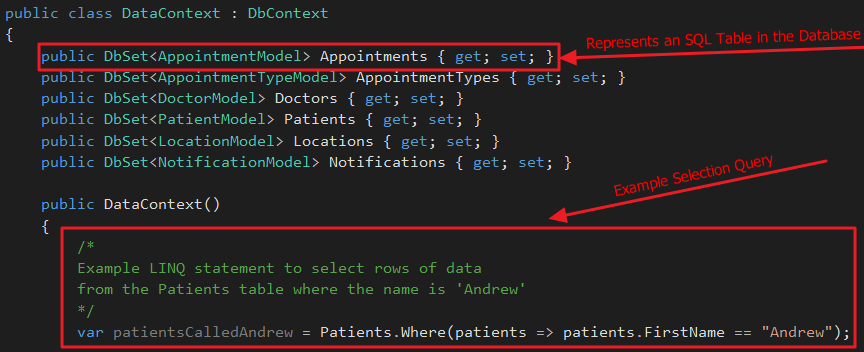
\includegraphics[width=\textwidth,height=\textheight,keepaspectratio]{Figures/EFContext.png}
		\rule{35em}{0.5pt}
		\caption[Example of the Entity Framework Data Context]{Example of the Entity Framework Data Context}
	\label{fig:efcontext}
\end{figure}

Using LINQ allowed me to select data easily through code, removing the need for direct SQL queries which could over complicate the process and introduce security vulnerabilities.

\subsubsection{Migrations}

After data models are created and added to the data context, Entity Framework allows you to migrate sample data when using the code first method. Migrations were therefore used to insert sample data into the database, such as appointments, patients, doctors, locations and any other information required for the prototype to function.

Besides adding data to a database, migrations also generate the SQL code necessary for making alterations to a database, using a version control system to allow different revisions of the database to be created. This allowed me to manage and update my remote database easily and not worry about adding new tables manually.

\section{Client Structure}

The client application is composed of two separate code bases, the client core library and the Android application.

\subsection{Client Core Library}

The client core uses the component based design pattern and is responsible for the majority of the applications business logic. This includes:

\begin{itemize}
	\item Sending and receiving requests from the server
	\item Storing data in the phone's memory and allowing multiple views to access it easily.
	\item Writing data to the phone's internal sqlite database
	\item Any other logic that isn't a platform specific feature
\end{itemize}

The client core is accessed via a static reference which means a component can be retrieved easily anywhere in the application. This turned out to be very useful for storing information that needed to be accessed by multiple parts of the client application.

\subsubsection{Creating Requests}

Besides storing data, the client core was also responsible for sending and receiving data from the server. To do this, the client needs to create a request and send it to the server so that it can receive data in return.

A client request is composed of three parts, the request url, the request parameters and the request method.

\begin{figure}[htbp]
	\centering
		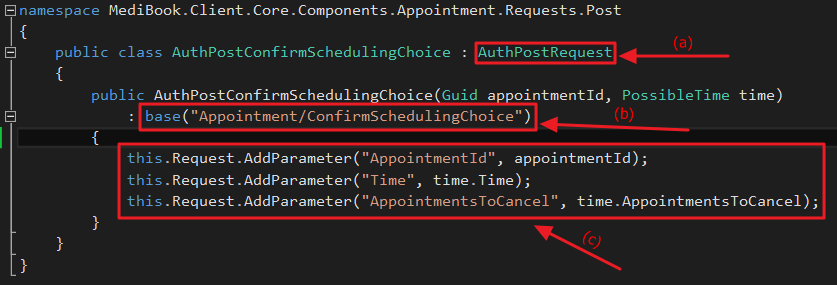
\includegraphics[width=\textwidth,height=\textheight,keepaspectratio]{Figures/ExampleRequest.png}
		\rule{35em}{0.5pt}
		\caption[Creation of a client request]{Creation of a client request}
	\label{fig:examplerequest}
\end{figure}

Figure \ref{fig:examplerequest} shows a request for confirming an appointment time with the server, specifying all three parts of the request.

Figure \ref{fig:examplerequest}(a) shows that this particular request extends the 'AuthPostRequest' which is retrieves the authorisation key from the account component and adds it to the request header. It also sets the request method to 'POST'.

Figure \ref{fig:examplerequest}(b) shows the request url, which it passes into the base constructor and is added to the request. This particular request targets the 'ConfirmSchedulingChoice' request method in the server's Appointment Controller.

Figure \ref{fig:examplerequest}(c) shows the parameters being added to the request. A parameter is a string key value pair which is added to the request so that it can be parsed by the server's request binding model.

\subsubsection{Request Response}

After the request has been created, the client executes it, sending it to the server and waiting for a response.

\begin{figure}[htbp]
	\centering
		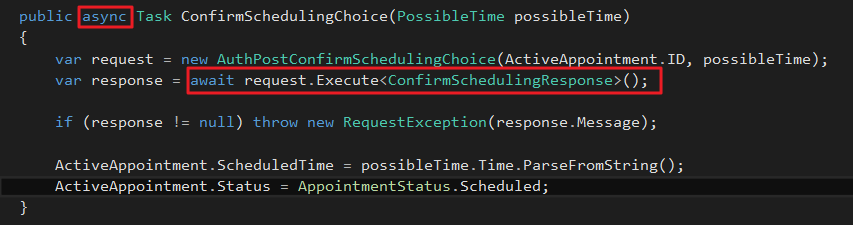
\includegraphics[width=\textwidth,height=\textheight,keepaspectratio]{Figures/ExampleResponse.png}
		\rule{35em}{0.5pt}
		\caption[Example of the client sending a request]{Example of the client sending a request}
	\label{fig:exampleresponse}
\end{figure}

In figure \ref{fig:exampleresponse}, you can see that the execution method also specifies a 'ConfirmSchedulingResponse' parameter. This is a binding model that the client then uses to de-serialise the response data into a usable form. This is similar to the server's implementation of the binding models and allows the specification of data types for the response data.

\subsubsection{Asynchronous Requests}

One problem I ran into when implementing requests was that my client application would halt until it received a response from the server (or the connection timed out). To solve this issue, I implemented asynchronous requests so that the program would continue functioning without waiting for a request to return its result first. This implementation uses the 'async await' feature in C\#. When the program hit's an await operator, the program will return to the request caller until a response is received. You can see this being used in figure \ref {fig:exampleresponse}.

This allowed me to effectively execute requests in the background without having an impact on the main application.

\subsection{Android Application}

The Android application, like the server application, uses the Model-View-Controller design pattern. The application structure was composed of a few base components; activities, intents, resources, layouts and services.

\subsubsection{Activities}

Android activities are the Android implementation of controllers. Usually tied to specific screens, they handle any logic required by the screen, including the creation of and switching to other activities if necessary.

Activities bind to an Android Layout and have several states that depend on if the activity is on the screen or not at the current time. For example, if the user presses the home button, the application is minimised and the activity is paused.

The Android client contained several activities, one for each screen available screen.

\subsubsection{Intents}

Android Intents are a description of a task to be performed. For example, when starting an activity, a 'StartActivity' intent must be created which takes the activity as a parameter. Intents are also useful for executing system tasks such as opening the phones dialer or calendar.

\subsubsection{Resources}

Android resources are all resources that the application uses, including pictures, layouts, sounds, constants and any other static data specific to the application.

As well as storing resources, the Android OS allows these resources to be easily accessed from within Activities.

The Android client uses resources to store all the layouts, fonts and images used in the application.

\subsubsection{Layouts}

Android layouts are views that define the visual structure for a user interface in the Android application.

Android provides an XML based API that corresponds to view classes and subclasses such as widgets that can be used in the user interface. It also allows you to attatch properties to these widgets that set it's position, id so the activity can find it, and many other variables that modify the widget's behaviour.

Xamarin also provides a drag and drop graphical user interface that allows for fast development of Android layouts for multiple devices.

\begin{sidewaysfigure}[htbp]
	\centering
		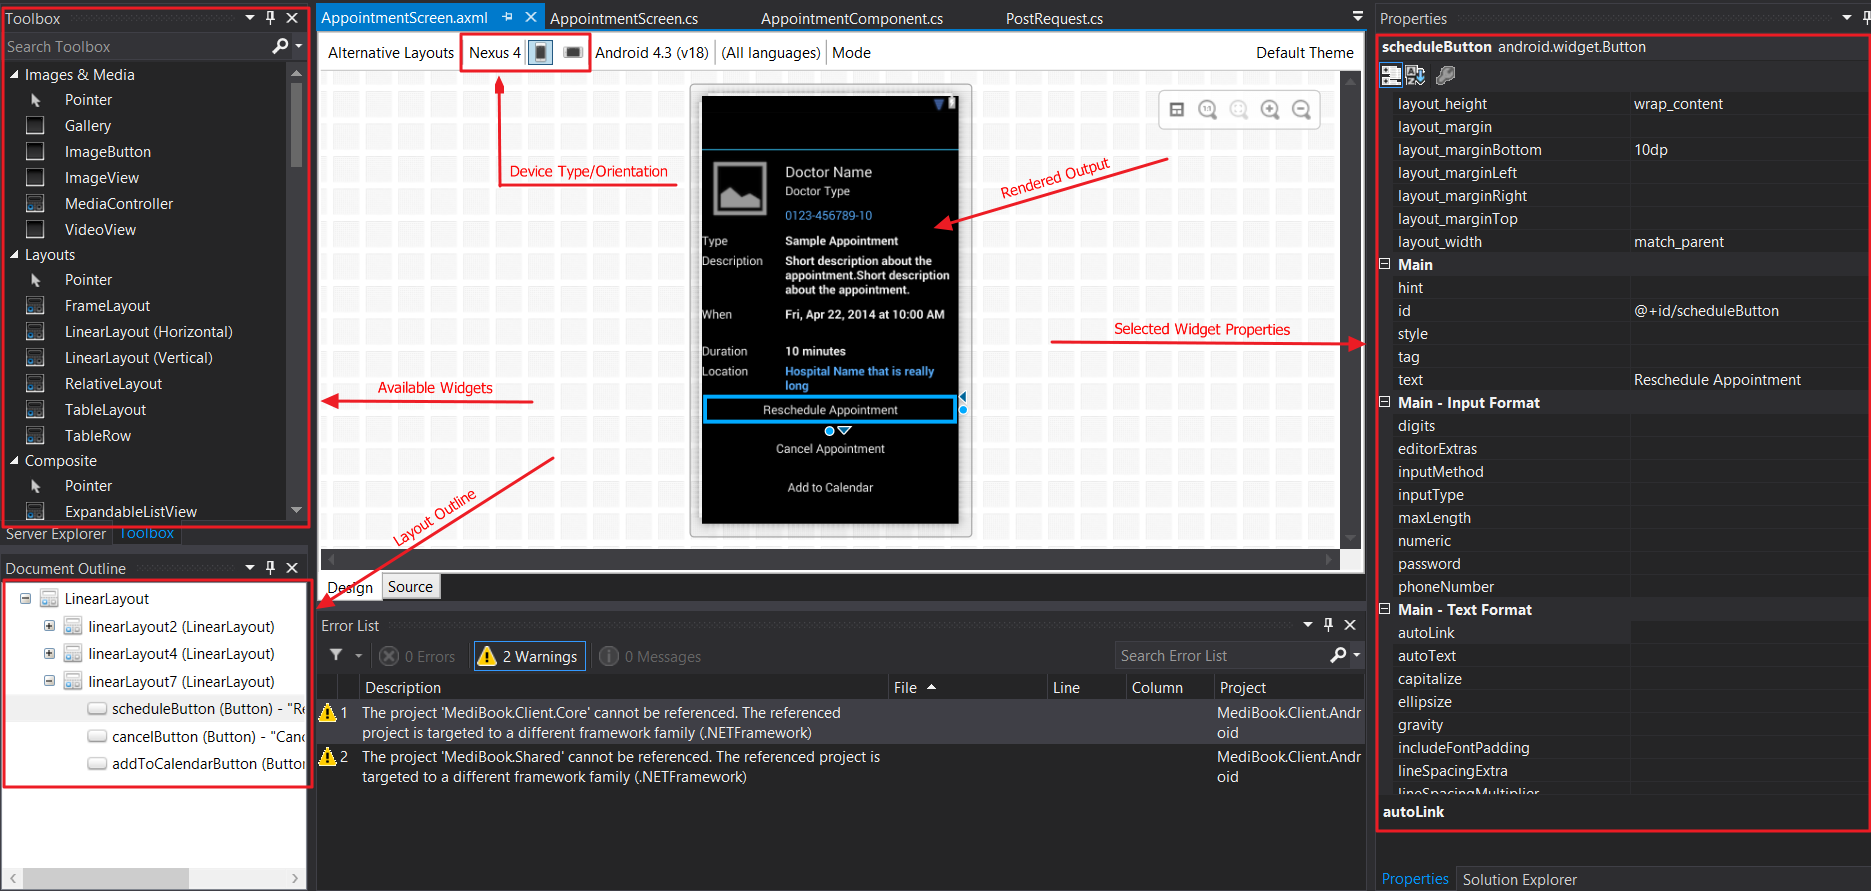
\includegraphics[width=\textwidth,height=\textheight,keepaspectratio]{Figures/XamarinLayoutDesigner.png}
		\rule{35em}{0.5pt}
		\caption[Screenshot showing the use of the Xamarin Layout Designer]{Screenshot showing the use of the Xamarin Layout Designer}
	\label{fig:layoutdesigner}
\end{sidewaysfigure}

As widgets are added to the design, the designer generates the XML source code for the layout. It also allows you to edit the layout code directly, re rendering any changes you make. This made it extremely useful as you did not need to compile and run the Android app (a process that can take a long time) every time you make a change to the design.

\subsubsection{Services}

Android services allow tasks to run in the background. They run in their own independent life cycle, meaning that they continue to function even when the app isn't running.

Android services were used to process incoming notifications sent from the google cloud messaging server. This allowed for the phone to receive messages whilst the app was not running and inform the user of changes to their appointments.

\section{Login and Authentication Feature}

With the basic infrastructure established, implementing the app authentication procedures was fairly simple.

To manage the authentication requests and logged in account, I created a component in the app core library which sends the login, registration and logout requests, as well as storing the current token used to sign authorised requests.

The Android visual implementation of this feature was also very straight forward. I created an activity and set it as the main launcher activity. This tells the Android OS to open this particular activity first when starting the app.

The login screen has two text input widgets that allows users to input their login details. Two buttons were also added which linked to the activity and sent the login and registration requests.

\subsection{Login Request}

The login request sends the user name and password input via the HTTPS protocol ensuring it is sent securely. If the login is successful, the server will respond with an access token, which is then stored in the account component.

\subsection{Registration Request}

When creating a new account, the following information is needed as parameters in the request:

\begin{itemize}
	\item UserName - unique user name required to log in with.
	\item Password - secret password required to log in with.
	\item AccountType - Either 'Patient' or 'Doctor'.
	\item FirstName
	\item LastName
\end{itemize}

Upon creating a new user account, the server will assign this account the role of either doctor or patient and add some example appointments to the account (for demonstration purposes). If the request is successful, the server responds the HTTP status code '200 OK'.

\subsection{Incorrect Input}

If either the login request or registration requests have incorrect input, the server will return the HTTP status code '401 Bad Request', also stating a reason as to why it failed such as 'Incorrect Password'. To give some feedback to the user, I needed to also implement an error text field in the layouts design which displayed when there was an error.

\subsection{Conclusion}

The login and authentication feature was surprisingly simple to implement due to the fact that Asp.Net has the majority of it built in. Combined with the role system, it made it very easy to identify users server side from the access token used to send the request, which became invaluable when deciding which appointments to send to the client.

I also found that because the login request was a perquisite for any further action of the app, I added a progress dialog widget which shows whilst the app is waiting for a response from the server. 

A dialog is a simple modal view, much like a pop up which displays data on top of the main layout. This simple visual feedback was effective at telling the user to be patient while the login request is in progress.

\section{Home Screen Feature}

For the home screen, two main features were required; the appointment list and the notification list. To allow for two separate lists on the same screen, the home screen was implemented as a tab activity.

\subsection{Tab Activity}

Tab activities allow easy navigation of two separate user interfaces and keep the design clear and separate. Navigation tabs are added to the top of the view in an action-bar to allow the user to easily switch between the different interfaces. 

To embed an interface into a tab, fragments must be created to host these interfaces. In this case, list fragments were used to display and manage the lists. The home screen layout then had a fragment container, which hosted the selected tab's corresponding fragment within it.

\subsection{Fragments}

Fragments are child activities that represent a portion of the user interface. Instead of embedding a layout into an activity, you can embed the layout into a fragment, and then add that fragment to an activity. This results in the ability to have multiple screens per activity.

\subsection{List Fragments}

By using the list fragment, I was able to create a layout design for a single item and assign it to an adapter.

Android adapters act as bridges between the layout and data for the view. This is required for a list fragment so that it knows how to bind the data to the layout correctly, allowing for dynamic lists to be created easily. It also adds functionality such as the order in which items appear in the list, as well as touch event handling to determine which item was selected.

By keeping a reference of the appointment/notification and it's index in the list, I was able to invoke a new activity with the relevant information needed when the user tapped on a list item.

\subsection{Retrieving Appointments}

Whilst implementing the client side, I used sample data to populate the data lists. Once the client implementation was complete, I started on implementing a request to fetch all of the appointments that are assigned to a patient.

\subsubsection{Server Side Request}

I started by creating a new controller in my server project to manage appointment requests, setting all requests in the controller to require authentication.

This allowed me to not only keep the information secure, but also fetch the patient's identity easily by using the Asp.Net property 'User.Identity' that is available in all authorised requests. The Asp.Net populates this by checking the used token against logged in sessions, retrieving the correct identity from the session.

\subsubsection{Appointment Model}

An appointment model was created based on my original ER Diagram and put in the shared project so that both the client and server could access it. This was to allow the server to store, retrieve and send the data to the client, as well as allowing the client to use the model to de-serialise the returned data from the request. 

The model was then added to the data context and a new reference of the data context was created within the appointment controller.

With the patient's user name available, it was very easy therefore to retrieve all appointments linked with that user name, returning them in the request.

Figure \ref{fig:efmodel} shows the appointment model and it's properties. Although not all of the information was relevant for the list, this query sent of the entire appointment model so that it could later be used in the Appointment Information Screen, removing the need for a second query to be executed.

\subsection{Action Bar}

With the relevant appointments being successfully retrieved from the server, the appointments were stored in the appointment component and injected into the list adapter.

Later on in the implementation, I found that these appointments were becoming out of date. I found that a good solution to this was to create a button to manually fetch appointments from the server and repopulate the list.

The list view took up the entire screen and I did not want to remove focus from it as it was the main feature, so I created a second action bar above the tab bar.

To implement this, I utilised the 'App Compat' Android library which adds a top bar menu to all your activities. This made it very simple to add button tabs at the top of your screen, as well as displaying the name of the current screen to make navigation of the app easier.

A refresh button was added which, when pressed, would request the appointment data from the server again. A rotating progress icon was also added to the button to show whilst the request was in progress. Another solution to ensure appointments were kept up to date was the adding of the request to the 'OnActivityResumed' method, which executes whenever the activity becomes visible again. This resulted in the app refreshing the appointments whenever the home screen was re-opened.

A logout button was also added to the bar to allow the switching of accounts and returned the user to the login screen.

\section{Appointment Information Feature}

With the appointments already retrieved, implementing the appointment information feature was simple. When a appointment was tapped on the list, it would set the 'CurrentAppointmentOpen' property to the relevant appointment in the appointment component. It then opened a new activity for the information screen.

To create the information screen, I used the layout designer to create a layout with the required widgets.

When the appointment information activity was started, it displayed the layout and retrieved the relevant appointment from the appointment component. It then assigned the text fields in the layout to the relevant information in appointment so that the information was specific to the requested appointment.

\subsection{Doctor's Image}

One technical challenge faced was providing the doctor's image for this feature. Images are normally added to the resources folder, however this would not be an effective solution because the app would then need to be updated whenever a new doctor is added.

Due to having a limitation on requests were only textual information could be sent, I added an image url to the doctor model. This url pointed to a web server hosting the image where by using a separate request, it could be retrieved.

Upon opening the activity, the image widget therefore contains a place holder image while it downloads the actual image onto the phone from the external server. This worked effectively and allowed doctor's portrait images to be changed remotely on the server without having to update the app.

\subsection{Buttons}

Several buttons were also created to allow the patient to easily schedule, re-schedule and cancel their appointments.

Upon pressing these buttons, the layout would invoke a method in the activity that carried out the functionality. The schedule button would create a new activity that took the user to the scheduling screen. The cancel button would send a cancel appointment request, sending the appointment id to the server in the request.

\subsection{Action Bar}

An action bar was also added to the appointment information screen using the same method as in the home screen. In the action bar, a map button was added that created a new activity for the map view, as well as a back button that finished the current activity and returned to the home screen.

\subsection{Dialer}

By tapping the contact number text field, the activity was required to open the phones dialer with the same number.

This was relatively simple to implement. The text field's 'OnClick' property was utilised to invoke an 'OpenDialer' method in the activity. This method created an Android Intent that told the Android OS to open the dialer action of the phone. The 'SetData' field to set the number from the appointment so that the dialer had access to the relevant information

One issue I had was that in order for the dialer to parse the number correctly, the string value passed to it must be prefixed with 'tel:', which was missed in the first iteration of it's implementation.

\section{Calendar Feature}

The calendar feature added a button to the appointment information screen, allowing the user to add (or remove) the appointment details to their phone calendar.

Accessing the phone calendar was a complex process, requiring Android app permissions, content resolvers to retrieve the information and extensive reading of poor Android documentation.

\subsection{Calendar Querying}

Android is a privilege-separated operating system, requiring all applications to request privilege permissions in the applications manifest. Certain restricted features are not available until these privileges have been added, which prompts the user upon the install of the application of the restricted features it has access to.

The app manifest is essentially the Android application's configuration file, specifying which android sdk version it uses and any permissions it requires. The calendar access required the permissions 'READ\_CALENDAR' and 'WRITE\_CALENDAR', prompting the user that the application was able to read and write from the calendar.

Content resolvers are used to manage access to a structured set of data in Android. One problem that content resolvers solve is data access conflicts, when multiple Android applications are modifying the same data at the same time.

As an added feature, I wanted to query the the calendar to see if the appointment was already added. This would allow me to swap the 'Add to Calendar' button with a 'Remove from Calendar' button.

To do this, I needed to create a content resolver to fetch the correct calendar id, and then create a second content resolver to check if any entries existed in that calendar.

\subsection{Issues}

This feature started out relatively simple, but became increasingly problematic because Android has lots of deprecated methods of accessing calendar information. Deprecated methods are old ways implementing a feature, but are left in the Android sdk to preserve backwards compatibility.

One issue I encountered was that upon removing an appointment from the calendar, I found that it still existed when I queried it. After reading different versions of the same Android documentation, I found the most up to date implementation and discovered that when removing an entry from the calendar, the latest version of Android sets a 'removed' field boolean to true rather than deleting the entry. Although this was very simple to fix (by checking this 'removed' field), it took me many hours to find out why my entries were not being deleted.

Another issue I encountered was that upon cancelling an appointment, it was not removed from the calendar, resulting in it displaying an incorrect time. This was fixed by calling the 'RemoveFromCalendar' method when an appointment time is updated.

\section{Location and Map Feature}

The location and map feature aimed to prevent patients getting lost on their way to the appointment. By tapping on the location name or selecting the map button in the action bar of the appointment information screen, the app opened the map activity.

The map activity was very simple to implement. Android has a 'MapFragment' class designed for embedding 'Google Maps' directly into apps, providing a dynamic map and useful helper methods to manipulate it. 

\subsection{Google Maps API}

To utilise the map fragment, Google requests that you provide your application API key in the app's manifest file. To obtain a key, you must register your app with google through the google developer portal, a process that takes just a few minutes, is free of charge and allows you to access many useful API's.

After adding the API key provided, the map fragment was able to render a map within the app.

\subsection{Placing a marker}

After implementing the app map, the solution required a marker on the map displaying the location position and name. This required me to change the location data model, adding latitude and longitude properties to it so that the server could send the correct location.

Once the marker was set on the map, the map's settings were changed so that the map view would open with the marker centred.

\section{Appointment Scheduling Feature}

The main feature of the application was the ability to schedule and reschedule appointments. This was the hardest feature of the project aside from the initial design. This was primarily down to the complexity of the scheduling process, resulting in many obstacles that needed to be avoided. To begin implementing feature, I created several workflow diagrams to emulate the scheduling of an appointment by hand. Different scenarios were drafted, providing a set of clear instructions that the server and client carried out for each one. By modeling out the scheduling process by hand, it made the implementation much easier.

\subsection{Date Picker}

To start scheduling an appointment, a button was added to the appointment information screen that invoked a schedule appointment activity. This activity had three buttons in it's layout; a time picker button, a confirmation button and a cancel button.

When selecting the time picker, a dialog was created that showed a date and time slider. Care was taken to ensure that the user could not pick a time before the current date. After the user had inputed a time and date, the confirmation button would execute the request.

\subsection{Example Scheduler}

To emulate a real world scheduling algorithm, I implemented an 'Example Scheduler' program to find an appointment for the user. The aim of this program was to return an appointment time as close to the requested time as possible. The first obstacle to overcome was appointment conflicts.

To detect conflicts, the scheduler queries the appointment database for all appointments where the times overlap. It first calculates the time range of the requested time using the appointment duration. If any scheduled appointments overlap, the scheduler will flag the time as conflicting. 

The scheduler deals with conflicts in two ways; using a priority based system to cancel other appointments or suggesting other available times. Every appointment is assigned a priority in the appointment model, based on how vital it is that this appointment is scheduled soon. This is used to compare how important appointments are relative to each other and whether an appointment can be rearranged or not.

If the conflicting appointments are less important than the requested appointment, the scheduler will cancel them and inform the patients and doctors by sending notifications to the devices. If the priorities are the same or the requested appointment is less important, the scheduler will find three possible times as close as possible to the requested time. It does this by incrementing the requested time hourly and repeating the conflict detection process again until it finds three possible appointments.

\subsection{Confirming the Appointment}

If the scheduler returns one result, the server will confirm the appointment and respond to the client that the appointment has been scheduled. Otherwise, it will return the three possible choices.

If three choices are received from the server by the client, the activity will start a new scheduling choice activity screen, which displays the times to the patient and asks them to choose one. Upon choosing a time, the client will send a confirmation request to the server to schedule the appointment.

\subsection{Time issue}

One issue I ran into when implementing this were time zones. The time calculated on the phone was in the time-zone 'British Summer Time (BST)', which was an hour ahead of the time calculated on the server 'Coordinated Universal Time (UTC)'. This caused many problems when sending and receiving times because they would become out of sync. 

My first attempt to solve this was simple, change the time zone that the server is running on. I later found that this was not possible because the server was hosted on the Windows Azure Cloud, designed to be run in any geographical location and therefore prohibiting any changing of the time-zone. The app had to be therefore designed to run in any time zone.

The second attempt to solve this utilised C\#'s 'TimeZoneInfo' class which allows for the conversion of times to different timezones. I later found that due to the nature of the the Monodroid compiler that allowed C\# to be transformed into Java based code, no regional information was available and the 'TimeZoneInfo' class was unable to function correctly.

I did not find a solution to this besides manually offsetting the between UTC and UTC + 1 when times are sent and received. This will not work forever, as when the phone's time zone changes from 'British Summer Time' back to 'Greenwich Mean Time (GMT)' the offset will still be in effect. However, as this was a prototype, this bug was not a priority.

\section{Notification Feature}

The last feature of the application implemented push notifications. The need for notifications was important for reminding patients about their appointments and providing live communication with them. Push notifications utilised the Google Cloud Messaging API to send the message and Android Services to process the messages as they are received.

Google Cloud Messaging was chosen to provide push notifications due to it's simplicity to implement, as well as being optimised for battery efficiency and poor bandwidth.

\subsection{GCM Service}

In order for the Android device to receive GCM messages, it must start a service that runs as a background process on the device. This service registers the application with the GCM Service that runs natively on all Android devices. Upon registration, a device registration id is provided which is used to determine which device to send the message payload to. This registration id must therefore be sent to the server and stored in the patients data model so that the server can successfully send messages to the correct device.

Besides device registration, the background service is also responsible for handling messages that are received from the GCM Server. Upon receiving a message, the 'OnMessage' method is triggered in the service with the resulting payload. This method adds the notification to the notification list in the home screen and shows creates a local notification to inform the user that they have a new message.

\subsection{Sending of GCM messages}

In order to create a GCM message, a rest request must be sent to the GCM servers. The request must contain the Android application's API key, the registration id of the patient's device and the message payload.

The API key is retrieved the same way as the Google Maps API key was retrieved, through the Google Developer Portal. This informs the GCM Service on the Android device which application the message is related to.

The registration id is sent via a web request from the Android app and the Account Component assigns this id to the relevant patient model. This means that no notifications can be sent to the device until it has retrieved this request from the Android client.

The message payload contains any data that is sent to the device, such as the notification message and the relevant appointment id. Different types of notifications are therefore created easily by specifying custom data in the payload.

\subsection{Observer}

Another important feature of sending notifications was the scheduling of them. Notifications need to be sent at specific times to remind patients about various aspects of the appointment. To do this, an Observer service was implemented on the Asp.Net server that runs in the background. This utilises the Timer method in the Observable class to execute notifications at a set time.

This allows for reminder notifications to be queued easily as an appointment is scheduled. The prototype automatically schedules a notification to be sent an hour prior to an appointment's start time.

%----------------------------------------------------------------------------------------